%%%%% Inspection and Characterization Plan for DESC

%----------------------------------------------------------------------------------------
%	PACKAGES AND DOCUMENT CONFIGURATIONS
%----------------------------------------------------------------------------------------

\documentclass[12pt, a4paper]{article}

\usepackage{graphicx} % Required for the inclusion of images
\usepackage{natbib} % Required to change bibliography style to APA
\usepackage{amsmath} % Required for some math elements 

\setlength\parindent{0pt} % Removes all indentation from paragraphs

%\usepackage{times} % Uncomment to use the Times New Roman font

%----------------------------------------------------------------------------------------
%	DOCUMENT INFORMATION
%----------------------------------------------------------------------------------------

\title{Inspection and Characterization Plan} % Title

\author{Science Release and Validation team} % Author name

\date{\today} % Date for the report

\begin{document}

\maketitle % Insert the title, author and date

\begin{center}
Version 0.1
\end{center}

% If you wish to include an abstract, uncomment the lines below
% \begin{abstract}
% Abstract text
% \end{abstract}

%----------------------------------------------------------------------------------------
%	SECTION 1 -- the document's purpose is described, plus reference info
%----------------------------------------------------------------------------------------

\section{Purpose of the document}

This document is aimed at describing the process to execute the test suite necessary to characterize new Rubin data releases, in the context of the DESC.

\begin{itemize}
\item The methods, tools and criteria (where applicable) to characterize and validate the Rubin dataset
\item The procedure for the execution of tests and inspection
\end{itemize}

%\subsection{Changes from the last version}

\subsection{Definitions, reference documents}

\begin{itemize}
\item Test run: a single execution of the whole SRV characterization framework. Includes tests using DESCQA, other sources, inspection of data and documentation.
\end{itemize}
 
%----------------------------------------------------------------------------------------
%	SECTION 2 -- the purpose of the test runs is described
%----------------------------------------------------------------------------------------
\section{Goals of the characterization process}

\begin{figure}[h]
\begin{center}
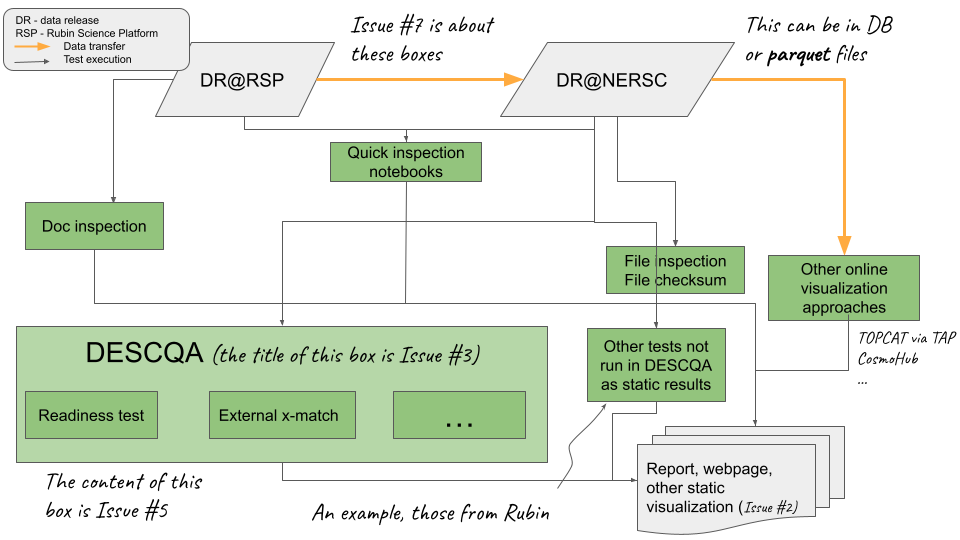
\includegraphics[width=0.95\textwidth]{../SRV_planning_diagram.png} 
\caption{SRV planning diagram}
\end{center}
\end{figure}


%----------------------------------------------------------------------------------------
%	SECTION 3 -- the software and other tools are described
%----------------------------------------------------------------------------------------

\section{Test tool description}

Here we include an overall view of the software involved in a single test run of the SRV characterization framework.

\subsection{Data sets and formats}

An explanation of the characteristics of the model of the data set being tested.

\subsubsection{DC2}

DC2 coadd catalogs is available as flat parquet files at NERSC.

\subsubsection{DP0.2}

TBC

%----------------------------------------------------------------------------------------
%	SECTION 4 -- the specific characterization cases and procedures are described
%----------------------------------------------------------------------------------------

\section{Characterization cases and procedures}

\subsection{Characterization of data set}
\subsubsection{TC1 - Inspection of catalog columns}
\textbf{Purpose:} Verify that the catalogs contain the columns we need
\textbf{Strategy:} Execute an interactive job over the whole data set of the ColumnInspection test from DESCQA.

This can be a simple listing of all columns, and making an automatic check on whether certain columns exist or not. 
Another part can check for NaNs or crazy values in the relevant columns (similar to what the Readiness test does in DESCQA)

\textbf{Procedure:} Describe how we actually go about running this (./descqarun --t ColumnInspection --c DC2 etc.)

\subsubsection{TC2 - Basic recursive characterization}
\textbf{Purpose:} Run a general 'readiness' test on coadd catalogs, to verify that there aren't any significant issues in data. 
\textbf{Strategy:} Execute an interactive job over the whole data set of the CoreChecks test from DESCQA.

The test currently comprises the following checks:
\begin{itemize}
	\item RA,DEC scatter plot
	\item Differential magnitude histograms in all bands, for PSF, aperture and model magnitudes.
	\item Magnitude vs magnitude error scatter plots of the above.
	\item Color-color plots (specifics TBC)
	\item Magnitude vs size plots fpr PSF-like objects
	\item PSF ellipticity whisker plot
	\item Source e1,e2 histogram (TBC, requires some source selection)
\end{itemize}

\textbf{Procedure:} Describe how we actually go about running this (./descqarun --t CoreChecks --c DC2 etc.)
%\textbf{Regression:}

\subsubsection{TC3 - Notebooks}
Interactive notebooks to be included here that complement or substitute DESCQA executions, that could be run on NERSC and RSP.

\subsection{TC4 - Inspection of external tests on same data set}
Add details of other test runs on the same data set that will complement this report: RAIL, faro, other analysis WG results.

\subsection{Inspection of available documentation}
This requires reporting where the documentation is available.

\subsection{Validation tests on small areas or subsamples, replicating previous scientific results}

%----------------------------------------------------------------------------------------
%	SECTION 5 -- the reporting is described
%----------------------------------------------------------------------------------------

\section{Test execution reports and visualization}

The reports should include date, DESCQA version (and other SW), data set version, people involved in the testing. Then the results would be a summary of an online resource where the complete collection of plots and numbers would be available.


\end{document}